\documentclass[letterpaper,12pt]{article}
\date{\today}
\title{Tetris part 4}
\usepackage{geometry}
\usepackage{graphicx}
\usepackage[tikz]{bclogo}
\usepackage{listings}
\geometry{left=2cm,right=2cm,top=1.5cm,bottom=1.5cm}
\usepackage[pdfusetitle]{hyperref}
\usepackage{xcolor}
\usepackage{newverbs}
\definecolor{codegreen}{rgb}{0,0.6,0}

\renewcommand{\verb}{\collectverb{\color{codegreen}}}

\begin{document}
\begin{center}
    \Large{Tetric Part 4}
\end{center}
To have a working Tetris, we need to complete a few methods.

\section{dropHeight(Piece, x)}
The \verb|dropHeight()| method should return y value of the piece's origin if it were dropped at the given column (x).

For example, in the figure below, the drop height of the piece is 2. Note it is not 3
even though it appears the bottom left of the piece sits on row 3. This is because the piece doesn't have anything at (0, 0)
but we are supposed to return the y value of the piece's bottom left position (0, 0).

You may want to draw a few diagrams and use the \verb|getSkirt()| method to help the calculation.
\\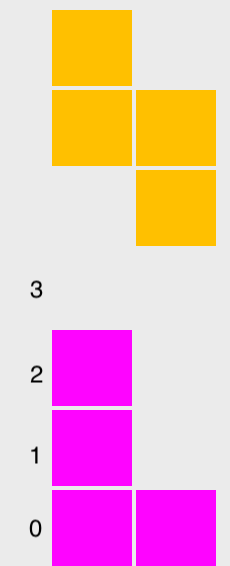
\includegraphics[scale=0.7]{drop.png}

\section{place()}

You should have implemented for the case of \verb|PLACE_BAD| and \verb|PLACE_OUT_BOUNDS| as well as \verb|PLACE_OK|. Now we need to implement the \verb|place()| method for the case of \verb|PLACE_ROW_FILLED|. This is the case where the row is filled after placing the piece.

This could be done by looking at all the rows to see if a row is filled with \verb|true| value in the grid.
 
\section{undo()}
This is very simple, we simply undo all the changed we did in the \verb|undoList|. Remember to clear the undoList after undoing,
otherwise, the undoList will keep growing in each place() call.

\section{commit()}
This means to commit the board grid with no undo available. This is simple, just clear the \verb|undoList|.

\section{clearRows()}
This is the most difficult method to implement. The idea is to clear all the filled rows and move the rows above down. This is done by looking at all the rows to see if a row is filled with \verb|true| value in the grid. If a row is filled, we should clear the row and move all the rows above down.

It could be done by having 2 pointers (indexes), \verb|i| and \verb|j|. \verb|i| starts from the bottom and iterate up. For each row of \verb|i|, if it is not filled, we copy the row to \verb|j| and increment \verb|j|. If it is filled, we skip the row without increment of \verb|j|. When we are done (up to the \verb|maxHeight|), we should fill the rest of the rows above \verb|j| with \verb|false|.

\paragraph{}

If you implement all the method correctly, you should have a working tetris game.

\end{document}
